\chapter{Stato dell'Arte}

\medskip

\section{Machine Learning}

Il Machine Learning (ML) \`e una sottodisciplina dell'intelligenza artificiale che \`e nata nel corso degli ultimi decenni del XX secolo. Nel campo dell'informatica, il ML \`e un'alternativa alla programmazione tradizionale, in cui a una macchina viene data l'abilit\`a di imparare autonomamente dai dati, senza richiedere istruzioni esplicite \cite{book_ML}. 
I metodi principali di apprendimento nel ML sono due \cite{ML_sup_unsup}:

\begin{itemize}

  \item \textbf{Apprendimento Supervisionato}: vengono utilizzati dati etichettati per effettuare il training del modello di ML. Nel set di dati \`e quindi associata un'etichetta ad ogni osservazione.
  
  \item \textbf{Apprendimento Non Supervisionato}: vengono utilizzati dati non etichettati durante l'addestramento. Non viene resa esplicita quindi nessuna relazione tra i dati, sar\`a l'algoritmo ad estrarre le informazioni necessarie a classificare o predire i risultati attesi tramite tecniche di clustering.
    
\end{itemize}

Nel nostro caso, abbiamo utilizzato l'apprendimento supervisionato avendo a disposizione dei set di dati etichettati.
Esistono principalmente due compiti dell'apprendimento supervisionato\cite{wiki_ML}:
\begin{itemize}

  \item \textbf{Classificazione}: un algoritmo (classificatore) \`e addestrato a classificare i dati di input su variabili discrete. Durante il processo di training questi algoritmi vengono esposti a dati di input, a ognuno dei quali \`e associata un'etichetta di classe e dovranno essere in grado, una volta addestrati, di restituire la classe di appartenenza di nuovi input forniti al modello.
  
  \item \textbf{Regressione}: un algoritmo (regressore) ha come scopo quello di individuare una relazione funzionale tra i dati di input e l'output. Il valore di output non \`e discreto come nella classificazione, ma \`e continuo.
    
\end{itemize}


\subsection{Algoritmi utilizzati}
Gli algortitmi utilizzati nel presente lavoro di tesi sono tutti classificatori, avendo preso come caso di studio un problema di classificazione, in particolare un problema di classificazione binaria e rilevazione di anomalie. Sono stati utilizzati in totale 4 algoritmi di classificazione, 2 per ciascuna classe di algoritmi:

\begin{itemize}

  \item \textbf{Algoritmi Statistici}: Logistic Regression, Linear Discriminant Analysis
  
  \item \textbf{Algoritmi basati su Alberi Decisionali}: Random Forest, XGBoost
    
\end{itemize}


\subsubsection{Algoritmi Statistici}
La \textbf{Logistic Regression (regressione logistica)} \`e uno degli algoritmi statistici pi\`u utilizzati nell'ambito del ML. Per regressione logistica si intende l'analisi di regressione che si conduce quando la variabile dipendente \`e binaria, ad esempio anomalia rilevata o non rilevata \cite{lr_rf}. L'algoritmo di regressione logistica pu\`o essere utilizzato per trovare la relazione tra una variabile binaria dipendente Y e una o pi\`u variabili indipendenti $X_{i}$. La Logistic Regression si compone delle seguenti variabili:
\begin{itemize}

  \item \textbf{Y, variabile dipendente binaria}: assume valore $0$ quando l'evento non si verifica (anomalia non rilevata) e valore $1$ quando l'evento si verifica (anomalia rilevata).
  
  \item \textbf{$X_{i}$, variabili indipendenti o regressori}: queste possono essere di qualsiasi natura, qualitative o quantitative e influenzano la variabile risposta Y.
    
\end{itemize}

\vspace{0.5cm}

Il modello da stimare \`e dato dall'espressione\cite{lr}:
\begin{equation}
P(Y=1 | X_1,...X_n) = \frac{1}{1 + e^{-(\beta_0 + \beta_1 X_1 + \beta_2 X_2 + \ldots + \beta_n X_n)}}
\end{equation}

Dove i coefficienti $\beta_0, \beta_1, \beta_2, \ldots, \beta_n$ sono i coefficienti di regressione

\begin{figure}[H]
    \centering
    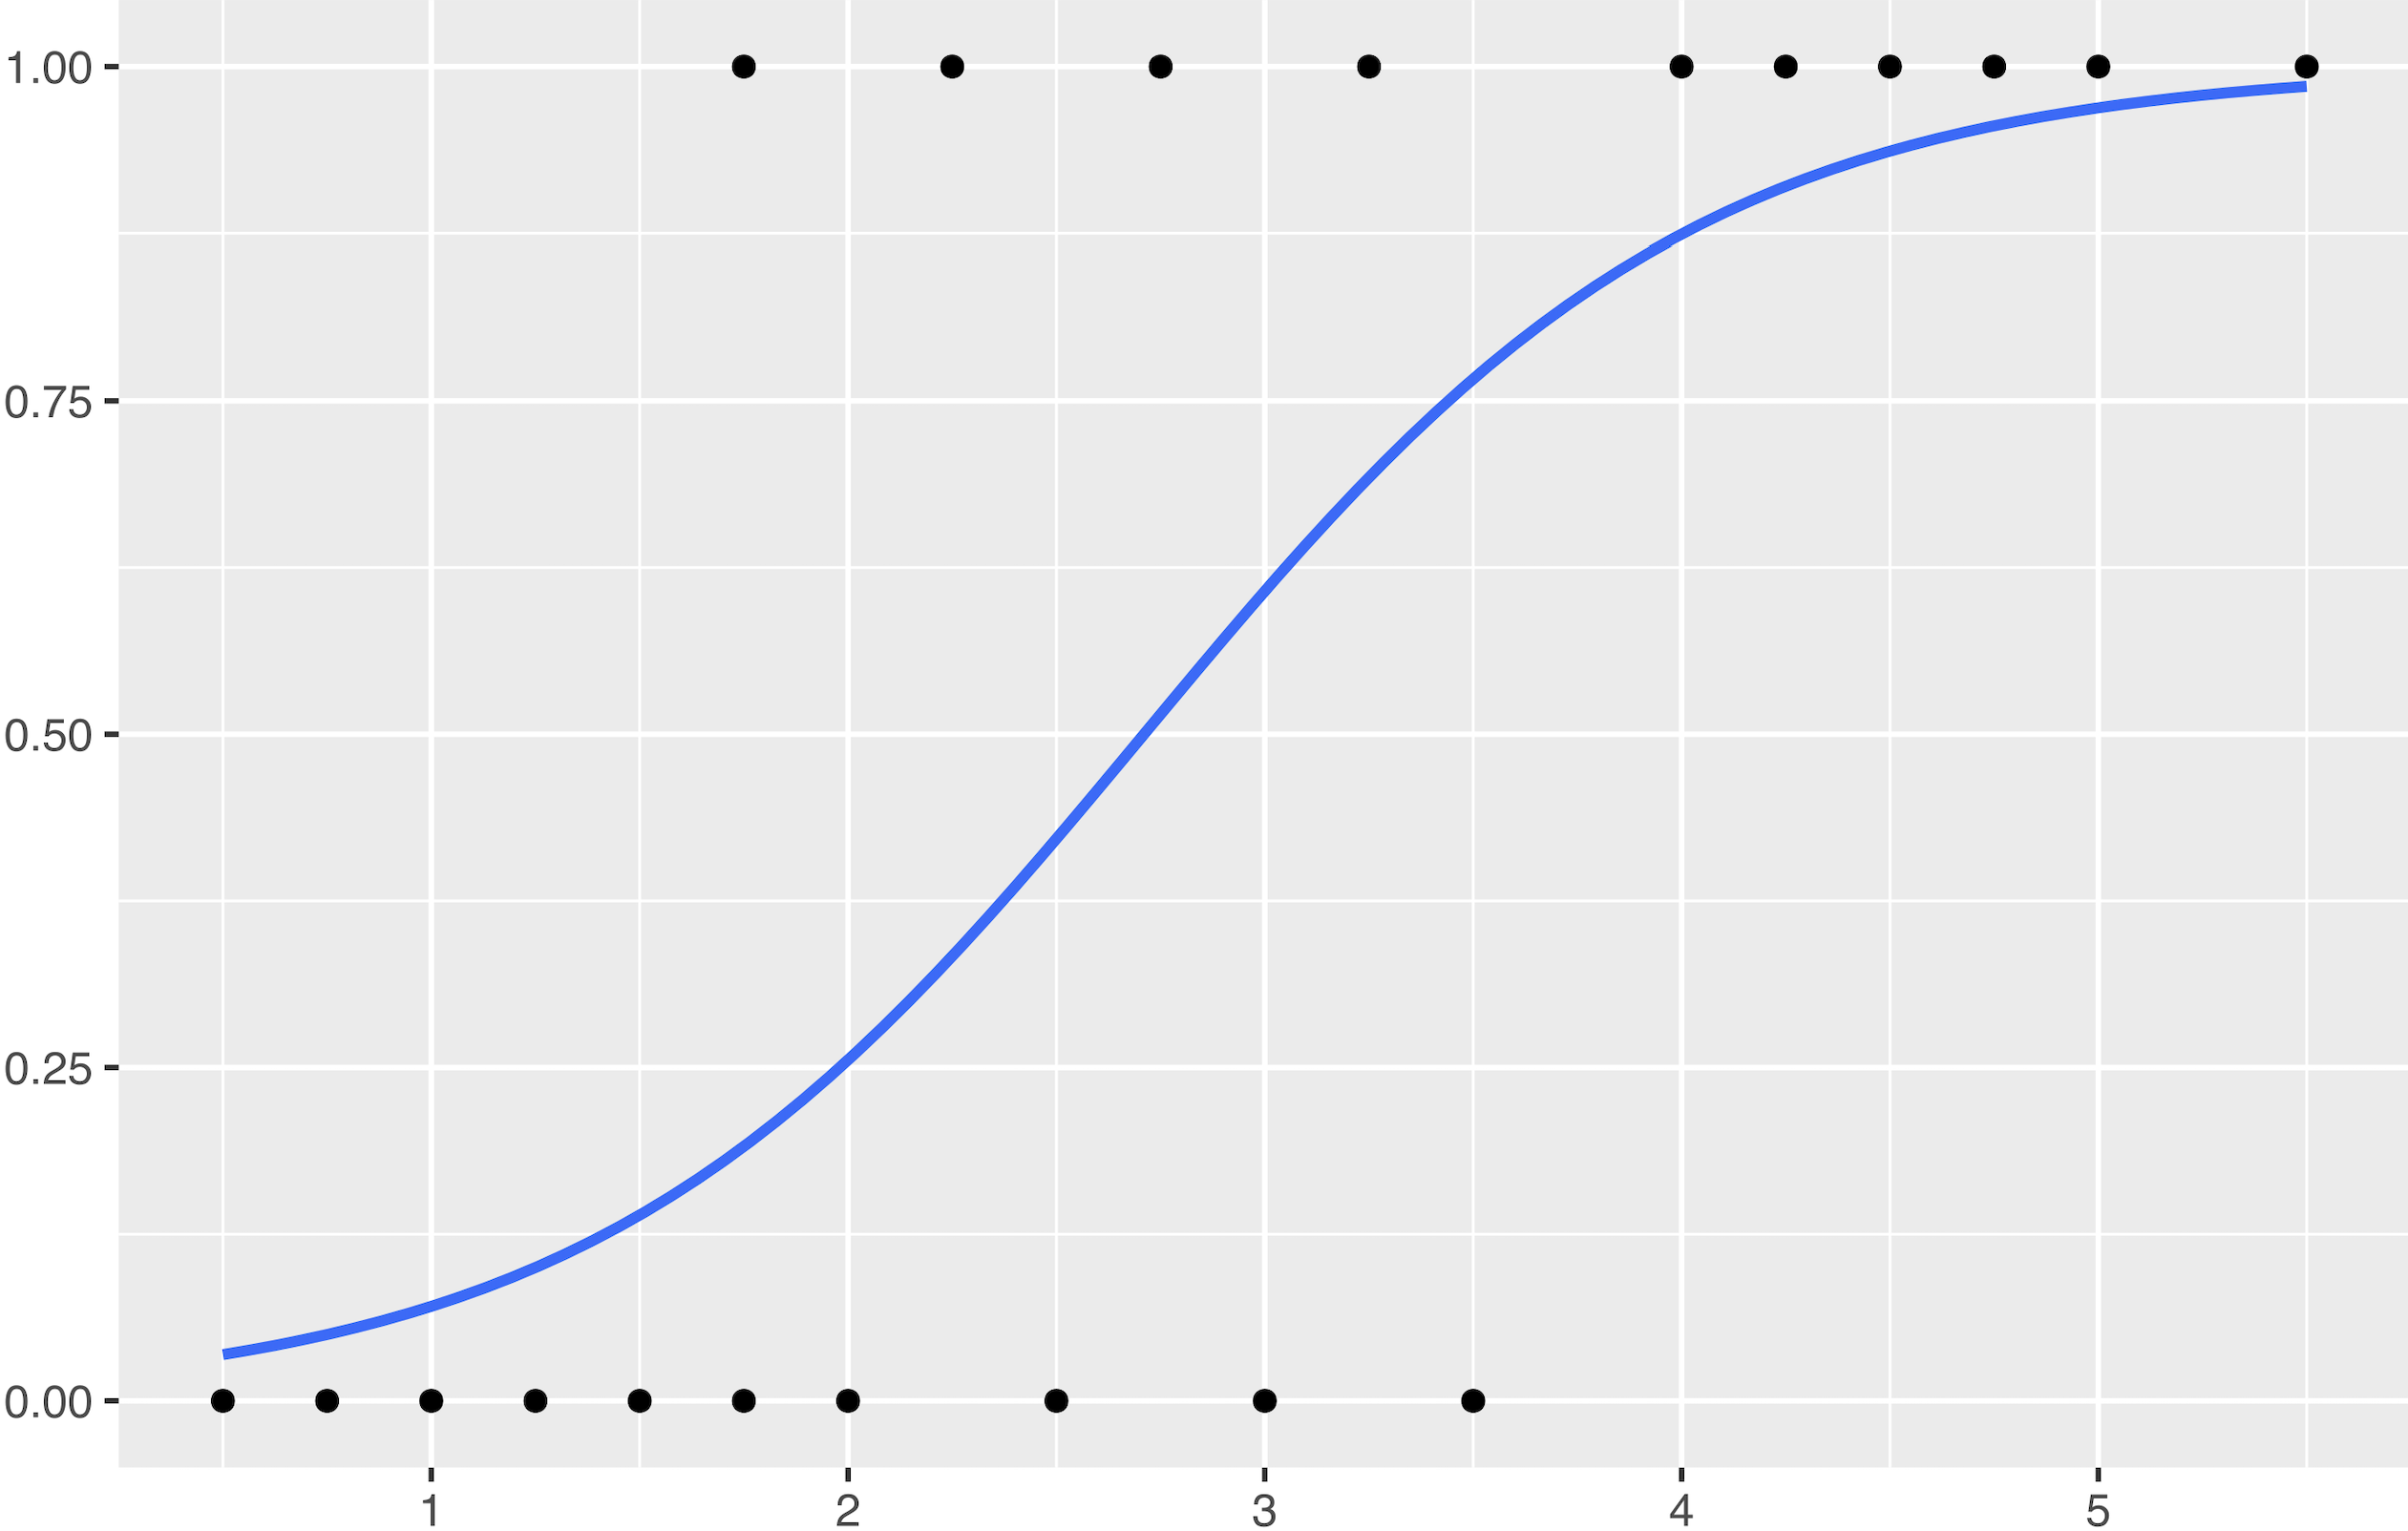
\includegraphics[width=0.6\linewidth]{Logistic Regression.png}
    \caption{Logistic Regression}
    \label{fig:logistic_regression}
\end{figure}

\vspace{1.5cm}

L'altro algoritmo statistico utilizzato \`e stato la \textbf{Linear Discriminant Analysis (LDA)}. Questo algoritmo, cerca di trovare una combinazione lineare di features che separino al meglio le classi nel dataset. La LDA funziona proiettando i dati su uno spazio a minore  dimensionalit\`a che massimizza la separazione tra le classi. Ci\`o avviene trovando un insieme di discriminanti lineari che massimizzano il rapporto tra la varianza inter-classe e la varianza intra-classe \cite{lda}. In altre parole, trova le direzioni nello spazio delle features che meglio separano le diverse classi di dati, nel nostro caso anomalia rilveata o non rilevata.

\begin{figure}[H]
    \centering
    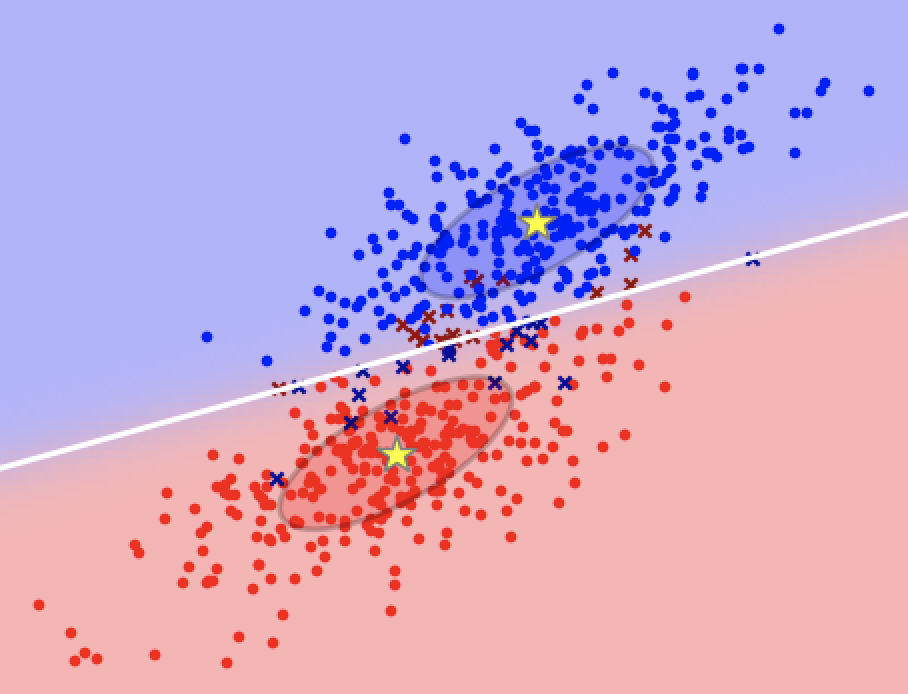
\includegraphics[width=0.5\linewidth]{LDA2.png}
    \caption{Linear Discriminant Analysis}
    \label{fig:lda}
\end{figure}

\subsubsection{{Algoritmi basati su Alberi Decisionali}}
Gli algortimi non statistici utilizzati sono entrambi basati sugli alberi decisionali, quindi prima di definire i singoli algoritmi, si proceder\`a con un'introduzione su cosa sono gli alberi decisionali. Un \textbf{Albero Decisionale (DT)} \`e un algoritmo ampiamente utilizzato nell'apprendimento supervisionato, adatto sia per attivit\`a di classificazione che per problemi di regressione. Questo algoritmo adotta una struttura ad albero gerarchica, caratterizzata da un nodo radice, rami, nodi interni e nodi foglia\cite{dt}.
\begin{figure}[H]
    \centering
    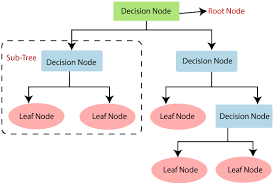
\includegraphics[width=0.6\linewidth]{DT.png}
    \caption{Schema Albero Decisionale}
    \label{fig:enter-label}
\end{figure}

\vspace{1cm}

Come rappresentato nel diagramma soprastante, un Albero Decisionale inizia con un nodo radice, che \`e contraddistinto dalla mancanza di rami in ingresso. I rami che si dipartono dal nodo radice alimentano i nodi interni, noti anche come nodi decisionali.  Sia il nodo radice che i nodi decisionali contribuiscono alla creazione di sottoinsiemi omogenei all'interno del dataset, in particolare, i nodi foglia rappresentano tutte le possibili previsioni o risultati nel set di dati. 
Il training dell'albero decisionale utilizza una strategia "dividi et impera" per cercare i punti di suddivisione ottimali all'interno di un albero.
Vediamo nella figura sottostante un diagramma, molto semplice e a titolo di esempio, di un albero decisionale per determinare la presenza o meno di un'anomalia all'interno di un calcolatore. 

\begin{figure}[H]
    \centering
    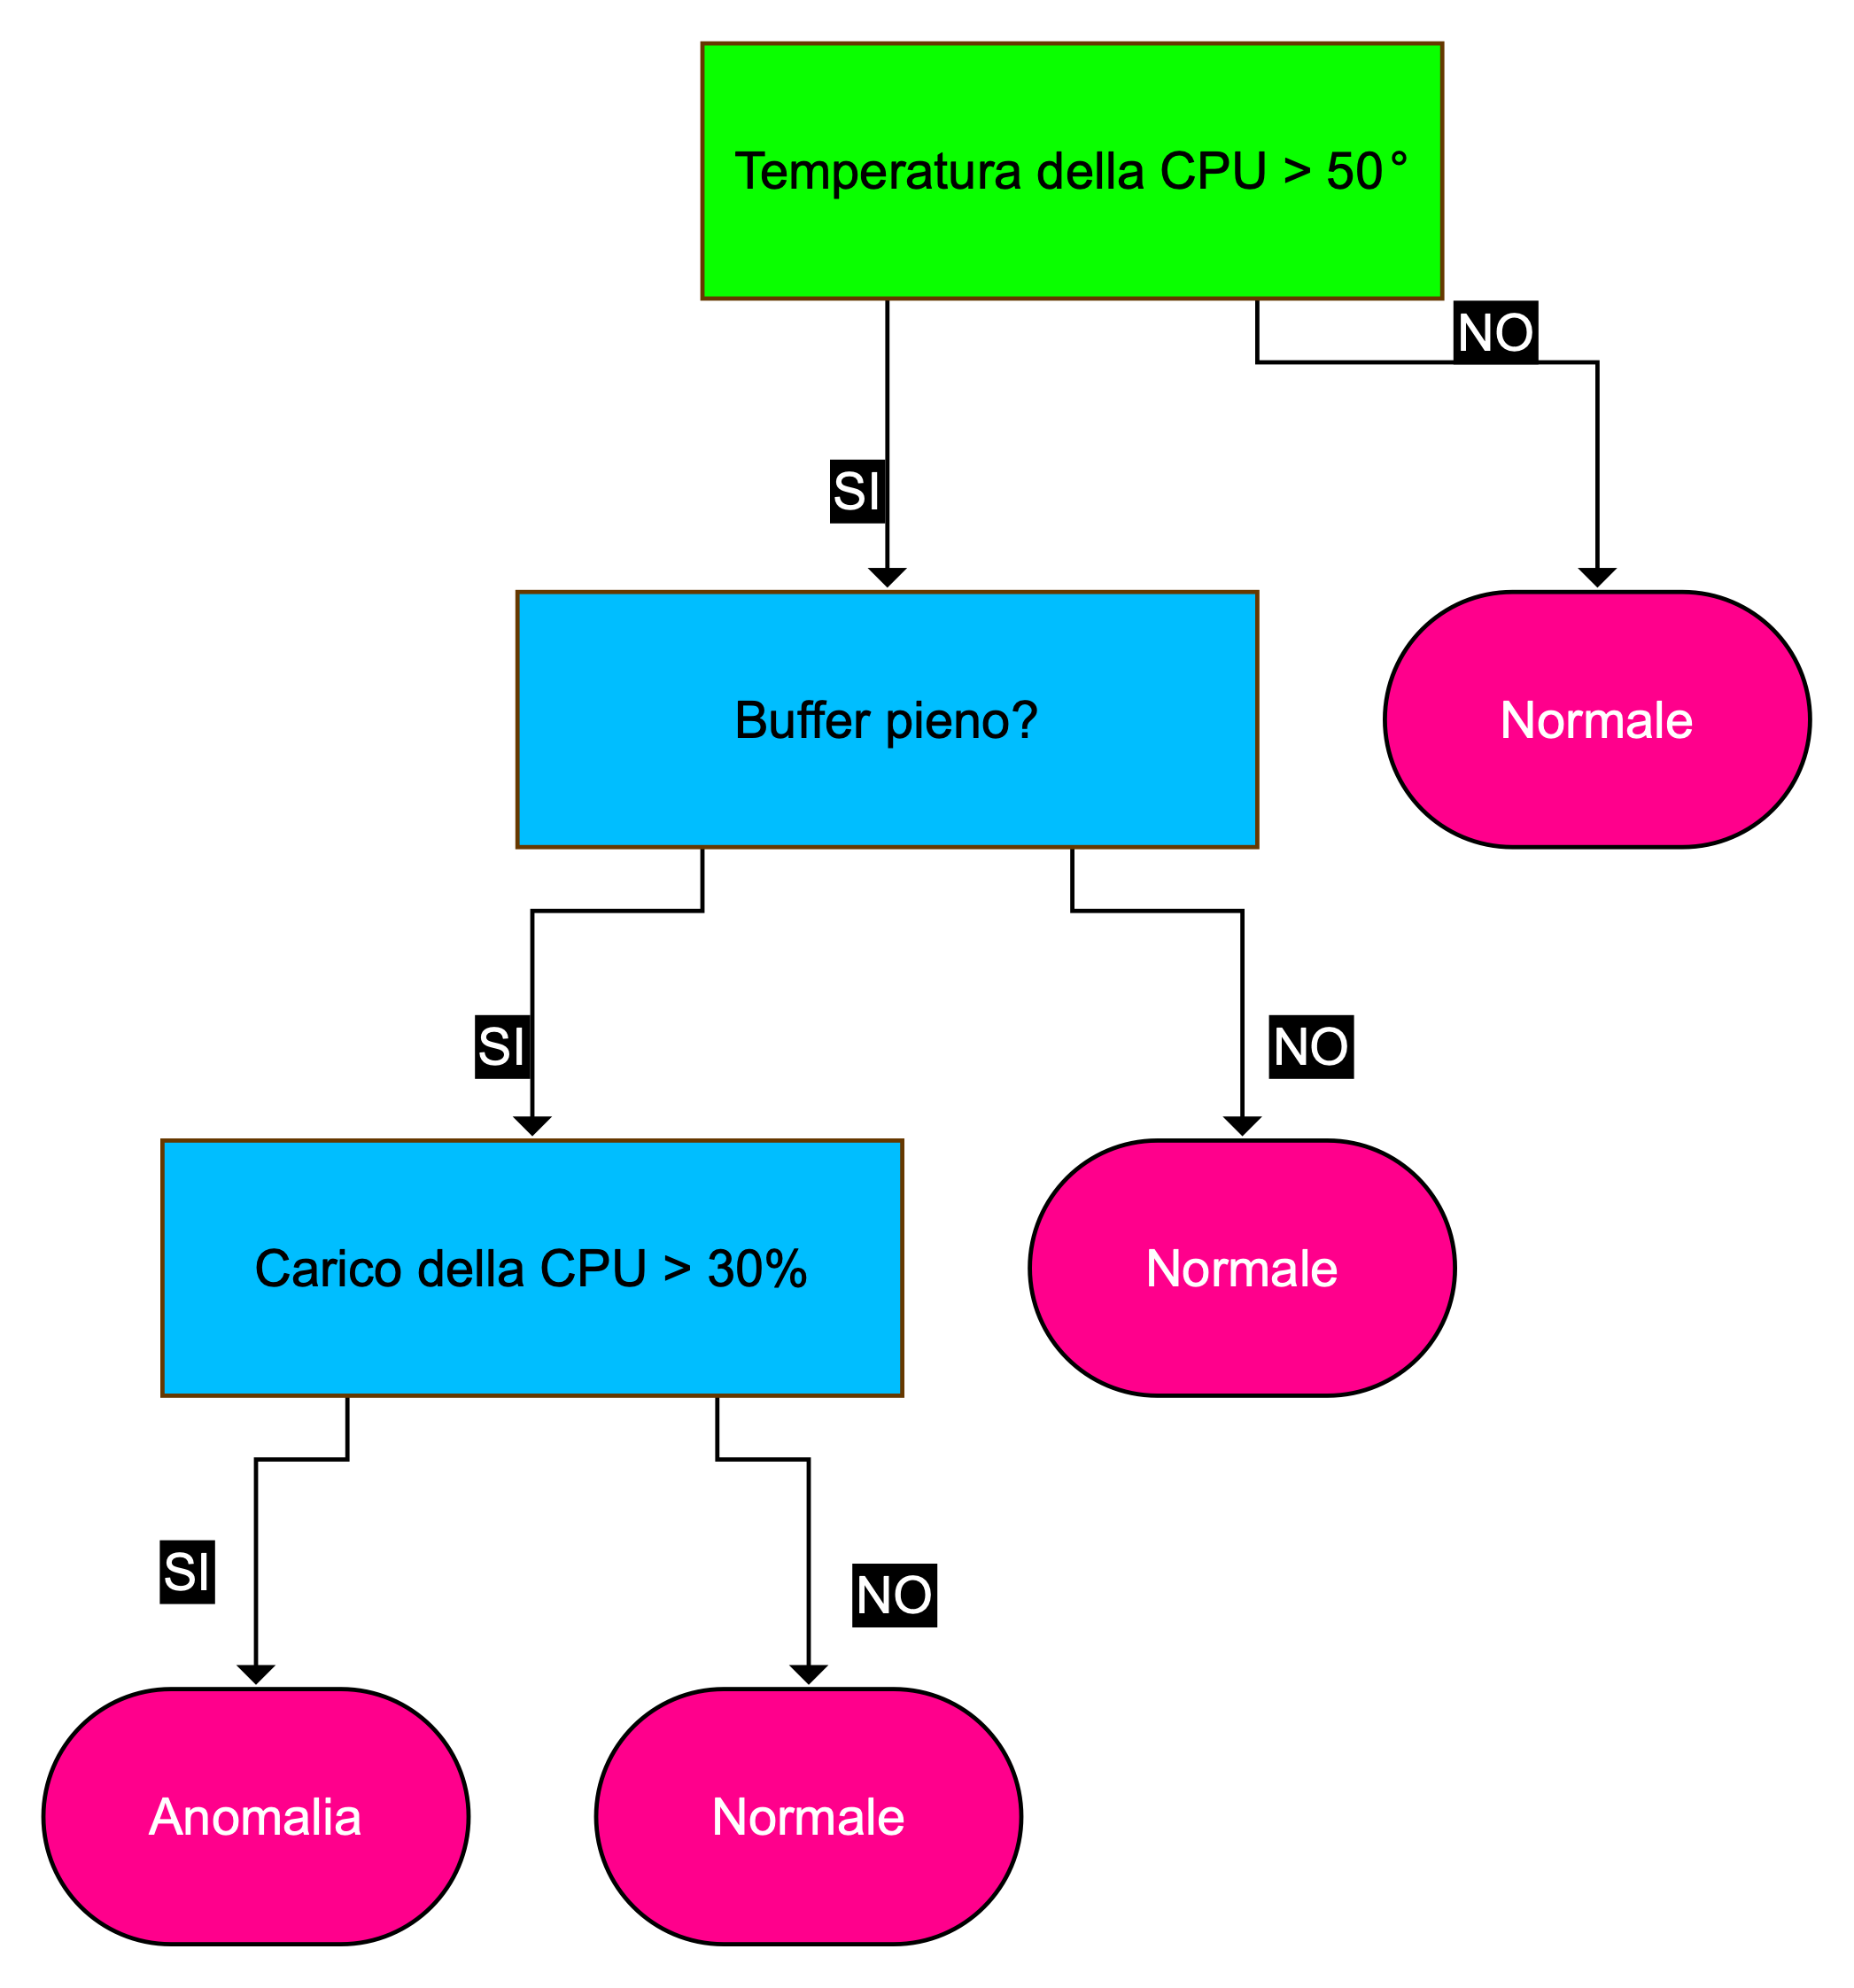
\includegraphics[width=0.6\linewidth]{Esempio DT.png}
    \caption{Esempio Albero Decisionale}
    \label{fig:enter-label}
\end{figure}

\vspace{1cm}

Nel nostro caso non sono stati usati direttamente degli alberi decisionali, ma degli algoritmi basati su di essi. L'algoritmo \textbf{Random Forest (RF)} \`e un classificatore d'insieme basato su alberi decisionali, ovvero \`e costituito da un insieme di classificatori, in questo caso DT, e le loro previsioni vengono aggregate per identificare il risultato pi\`u diffuso \cite{rf}.
In particolare, l'algoritmo RF utilizza una tecnica dell'apprendimento d'insieme, chiamata bagging, in cui pi\`u DT vengono addestrati su insiemi di dati diversi, ciascuno ottenuto dal dataset di addestramento iniziale. La casualit\`a delle caratteristiche su cui vengono addestrati i singoli alberi della foresta garantisce una bassa correlazione tra le singole strutture ad albero, riducendo cos\`i uno dei maggiori problemi degli alberi decisionali, l'overfitting. 
L'overfitting \`e un problema che si verifica quando un modello si adatta esattamente ai suoi dati di addestramento. Quando questo accade, il modello non funziona correttamente in presenza di dati non osservati in precedenza e non \`e quindi in grado di generalizzare, risultando inutile.
Possiamo schematizzare il comportamento dell'algoritmo Random Forest nella figura seguente.

\begin{figure}[H]
    \centering
    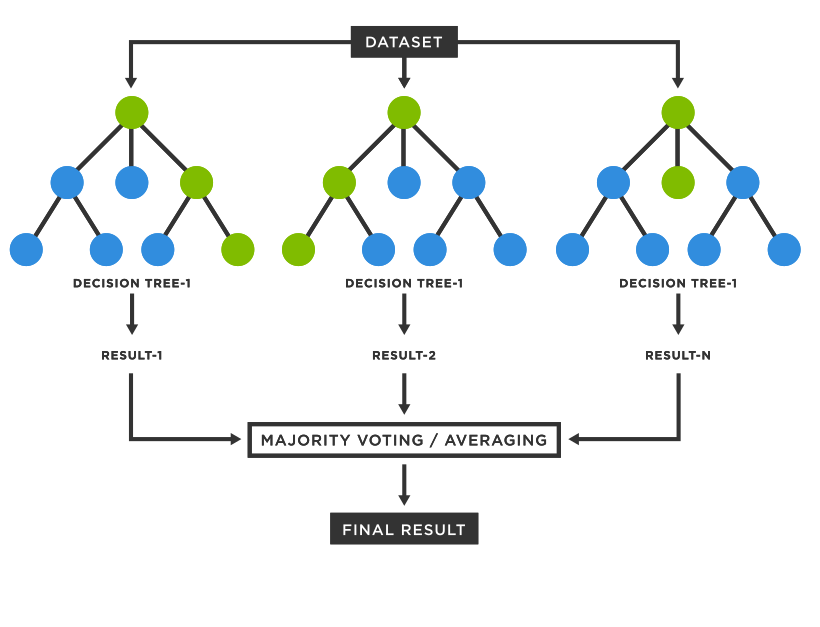
\includegraphics[width=0.6\linewidth]{RF Diagramma.png}
    \caption{Schema Random Forest}
    \label{fig:enter-label}
\end{figure}

Nel nostro caso, ovvero nel caso della classificazione, il risultato del modello corrisponder\`a al voto di maggioranza dei singoli alberi sulla classe prevista.

\vspace{1.7cm}

L'altro algoritmo basato su alberi decisionali utlizzato nel presente lavoro di Tesi \`e \textbf{XGBoost}, il cui nome completo \`e Extreme Gradient Boosting. Solitamente l'approccio pi\`u frequente quando si costruiscono dei modelli predittivi \`e addestrare un singolo modello forte. Un approccio differente potrebbe essere quello di costruire un insieme di modelli deboli che combinati costruiscano una previsione d'insieme forte. Quest'ultima idea \`e alla base di tutti gli algoritmi di ensemble learning, quindi anche di XGBoost e Random Forest \cite{gradient_boost}.
Come si deduce dal nome dell'algoritmo, XGBoost \`e basato sul boosting, ovvero un metodo di apprendimento d'insieme, proprio come lo \`e il bagging per Random Forest. Il boosting combina una serie di modelli deboli che vanno a formare un modello forte per ridurre al minimo gli errori di addestramento \cite{xgb}. Nel boosting, viene effettuata una selezione casuale dal set di dati e il modello viene addestrato in modo sequenziale, ovvero ogni modello successivo nella sequenza cerca di migliorare rispetto al precedente. I modelli deboli, che non sono nient'altro che alberi decisionali, vengono combinati per ottenere una previsione d'insieme forte. La differenza principale con la tecnica di bagging utilizzata da Random Forest \`e che nel bagging i modelli deboli sono addestrati in parallelo, mentre nel boosting apprendono in sequenza. Il miglioramento dei modelli durante l'apprendimento sequenziale avviene grazie all'algoritmo di discesa del gradiente (notare il termine \textit{Gradient} in  \textit{Extreme Gradient Boosting}), ovvero un algoritmo di ottimizzazione molto utilizzato nel ML.
XGBoost (Extreme Gradient Boosting) \`e un'implementazione di Gradient Boosting, nome utilizzato poich\'e combina l'algoritmo di discesa del gradiente e il metodo di boosting, progettata per velocit\`a e scalabilit\`a.


\subsection{Metriche di valutazione}
In questa sezione illustriamo le metriche di valutazione utilizzate per analizzare le performance dei modelli. Prima di menzionare le singole metriche, \`e necessario introdurre il concetto di \textit{confusion matrix (matrice di confusione)}. La matrice di confusione \`e una matrice utilizzata per valutare le prestazioni di un algoritmo di ML, che pu\`o essere cos\`i schematizzata \cite{mcc}:

\begin{figure}[H]
    \centering
    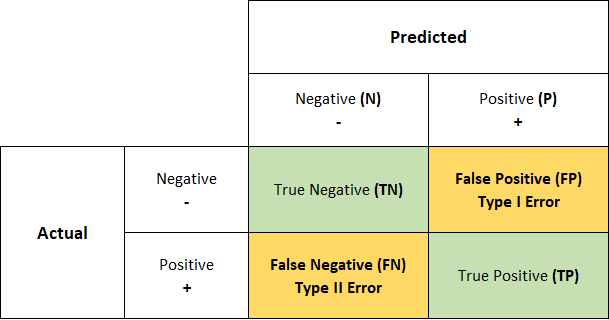
\includegraphics[width=0.5\linewidth]{confusion_matrix.png}
    \caption{Confusion Matrix}
    \label{fig:enter-label}
\end{figure}

Ora che abbiamo introdotto la confusion matrix possiamo meglio definire le metriche di valutazione. In totale sono state utilizzate 3 metriche di valutazione:

\begin{itemize}

  \item \textbf{Accuracy (ACC)}: il valore \`e dato dal numero delle classificazioni corrette diviso il numero totale di classificazioni. Formalmente, guardando alla confusion matrix, il valore \`e dato da:

  \begin{equation}
    ACC = \frac{TP + TN}{P + N}
  \end{equation}
  
  \item \textbf{Error Rate (1-ACC)}: il valore \`e dato dalla differenza tra 1 e l'Accuracy, ovvero $1-ACC$
  
  \item \textbf{Matthews correlation coefficient (MCC)}: questa metrica di valutazione, rispetto alle precedenti, \`e sicuramente la pi\`u robusta per valutare le performance dei modelli. Questo perch\'e, a differenza dell'accuracy, questa metrica non \`e affetta dal problema degli \textit{unbalanced datasets (set di dati sbilanciati)}, ma torneremo su questo problema tra poco. Guardando alla matrice di confusione il valore dell'MCC \`e dato da:
  
  \begin{equation}
      MCC = \frac{TP \cdot TN - FP \cdot FN}{\sqrt{(TP + FP)(TP + FN)(TN + FP)(TN + FN)}}
  \end{equation}
\end{itemize}

\vspace{1.5cm}

Riprendiamo il problema degli unbalanced datasets. Questo problema avviene quando, in una classificazione binaria, ad esempio,la frequenza di una delle due etichette risulta sbilanciata rispetto all'altra, ovvero una delle due etichette risulta molto pi\`u frequente nel dataset rispetto all'altra. Per comprendere al meglio il problema facciamo un esempio che risalti gli aspetti critici degli unbalanced datasets. Supponiamo di avere un dataset dove il 95\% dei dati \`e etichettato come 'normale', mentre il restante 5\% \`e etichettato come 'anomalia'. Se avessimo un modello chiamato \textit{dumb model} che classifica come 'normale' tutti i dati in input, avrebbe un'ACC del 95\% sul nostro dataset. Se prendessimo l'ACC come metrica di riferimento, il nostro \textit{dumb model} sembrerebbe un ottimo classificatore di anomalie, quando a stento potremmo definirlo classificatore. Abbiamo preso quindi l'MCC come metrica di riferimento perch\'e molto pi\`u robusta, non risentendo degli effetti dei set di dati sbilanciati.
    
\begin{figure}[H]
    \centering
    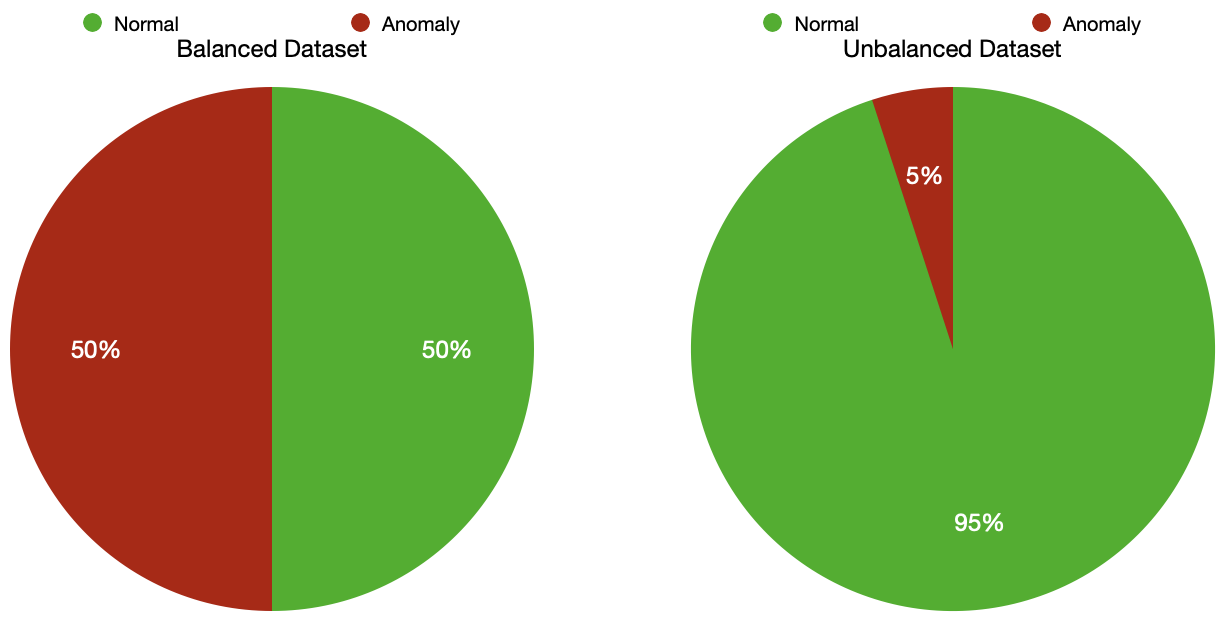
\includegraphics[width=0.7\linewidth]{Balanced_Unbalanced_Dataset.png}
    \caption{Balanced e Unbalanced Datasets}
    \label{fig:enter-label}
\end{figure}

\vspace{1cm}

\section{Anomaly Detection}
L'\textit{Anomaly Detection} (o \textit{rilevamento di anomalie} in italiano) consiste nella rilevazione di eventi rari che non rientrano nella definizione di comportamento normale dei dati \cite{anomaly}. Il rilevamento di anomalie \`e particolarmente importante nel settore della sicurezza informatica, ma anche nei settori quali finanza, medicina e molti altri ancora. 


\begin{figure}[H]
    \centering
    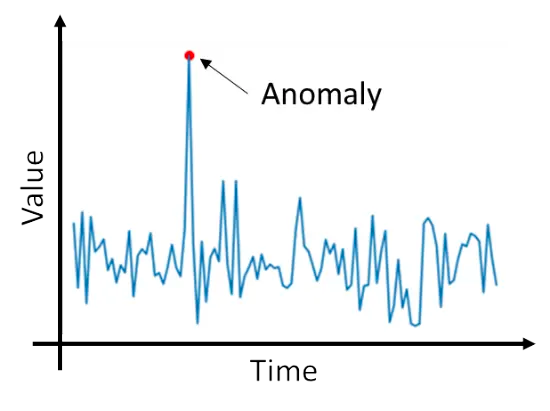
\includegraphics[width=0.6\linewidth]{anomalie.png}
    \caption{Esempio Anomalia Puntuale}
    \label{fig:enter-label}
\end{figure}


Un tempo chi si occupava di anomaly detection era solito eseaminare manualmente i dati, alla ricerca di comportamenti fuori dal normale, spesso non trovando le cause principali delle anomalie. Ad oggi il rilevamento di anomalie si basa quasi totalmente sul machine learning. Per definizione le anomalie sono eventi rari e quindi avremo a che fare spesso con dataset sbilanciati, con maggior presenza di dati etichettati come 'normali' rispetto a quelli etichettati come 'anomalie'.

\section{Time Series}
Il tempo \`e una variabile fondamentale per fare delle previsioni sul futuro. Per introdurre questo fattore nei nostri modelli ricorriamo alle \textit{Time Series}(o \textit{serie storiche} in italiano), che vengono definite come un insieme di osservazioni ordinate rispetto al tempo \cite{time_series}. L'analisi delle serie storiche non coincide meramente con l'atto di raccogliere e analizzare dati nel tempo. Ci\`o che contraddistingue una serie strorica da altri tipi di dati \`e che in una serie storica \`e possibile vedere come le variabili o features cambino nel tempo. Il tempo \`e una variabile cruciale e fornisce delle informazioni aggiuntive per i modelli.
Le serie storiche vengono solitamente analizzate con modelli specifici per \textit{time series forecasting}, che consiste nell'utilizzare un modello per predire valori futuri basandosi sui valori precedentemente osservati. In letteratura, difficilmente vengono utilizzati algoritmi di ML come Random Forest o XGBoost per l'analisi di serie storiche \cite{time_series_link}. Quello che ci siamo proposti in questo lavoro di Tesi \`e stato unire un problema di classificazione binaria (Anomaly Detection Supervisionata) con un approccio time series per dare maggiori informazioni ai modelli in fase di training, aspettandoci un miglioramento nelle performance dei modelli stessi.

 \vspace{-0.5cm}
 \vspace{-0.3cm}
